% Provenance (never printed): cycle 4 SVT/physique, "La planete Terre,
% l'environnement": uneven heating of the Earth, movements of the
% atmosphere, the global circulation and the climate zones; see
% sources/book1/PROVENANCE.md. Book 1, grade 8, chapter 2.
% Vocabulary guard: owns convection cell (atmospheric, descriptive), sea
% breeze and land breeze, the global winds, the global circulation. The
% Coriolis effect is told as "the Earth's rotation deflects"; Hadley and
% Ferrel cells and the intertropical convergence zone are named in prose
% only (Book 3 owns them); mantle convection is Book 2's.
\chapter{Los vientos y la circulación general}\label{ch:g8:winds-global-circulation}

Durante siglos, los veleros que salían de los puertos de Europa y de África
hacia América contaron con un viento constante del este, que sopla a ambos
lados del \omterm{def:g3:continents-and-oceans:equator}{ecuador} y los llevaba a través del Atlántico. Los marinos de todo
el mundo lo conocían, y el primer comercio con América dependía de él: es
el \emph{alisio}. Todavía hoy, los barcos de carga aprovechan los \omterm{def:g8:winds-global-circulation:global-winds}{alisios},
y las corrientes oceánicas que estos impulsan, para acortar sus travesías.
% ledger: nos:trade-winds

\begin{omfigure}
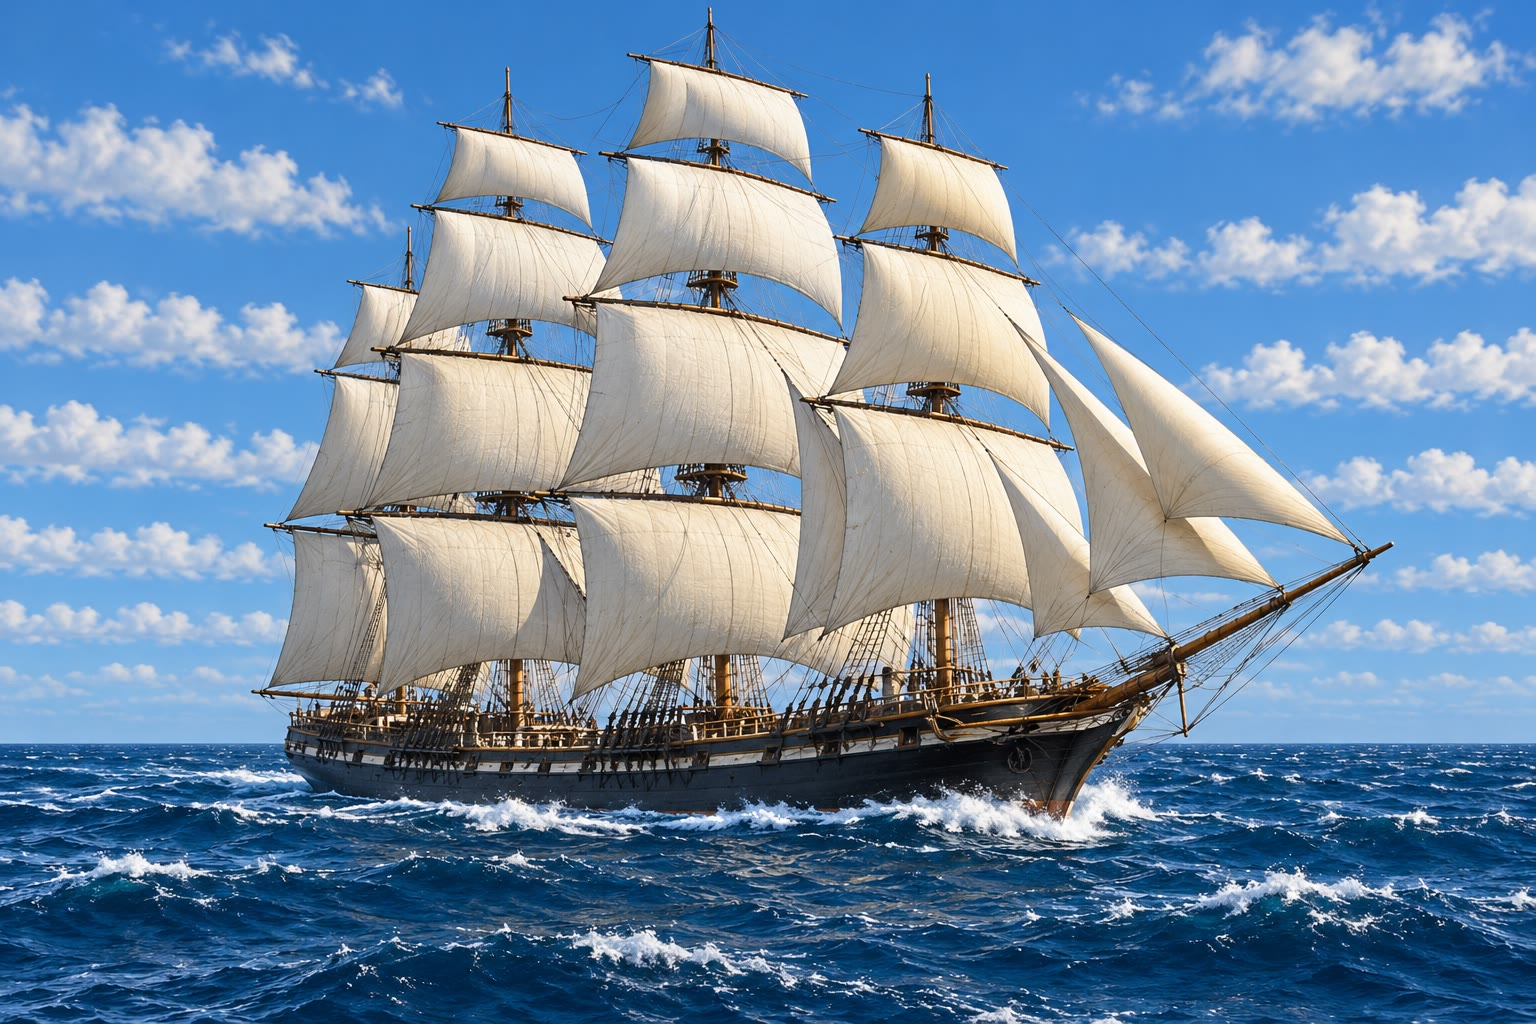
\includegraphics[width=0.62\linewidth]{images/book1/ai/g8-sailing-ship.jpg}

{\small Un velero navega empujado por un viento constante en alta \omterm{def:g2:water-on-earth:ocean}{mar}
(ilustración generada por IA de una escena genérica).}
\label{fig:g8:winds-global-circulation:ship}
\end{omfigure}

¿Por qué el alisio sopla del este, y siempre en los mismos lugares? ¿Por
qué hay \omterm{def:g5:weather-and-climate:desert}{desiertos} cerca de los \omterm{def:g5:weather-and-climate:tropics}{trópicos} y \omterm{def:g5:weather-and-climate:rainforest}{selvas tropicales} cerca del
\omterm{def:g3:continents-and-oceans:equator}{ecuador}? La respuesta empieza por el Sol.

\begin{recall}
El viento es aire en movimiento (los libros de física). El aire presiona
sobre todo lo que toca, y la presión disminuye con la altura
(\cref{ch:g8:the-atmosphere}). El \omterm{def:g1:watching-the-weather:weather}{tiempo} meteorológico ocurre en la
\omterm{def:g8:the-atmosphere:layers}{troposfera}, la capa más baja de la atmósfera. La Tierra tiene \omterm{def:g5:weather-and-climate:climate-zone}{zonas
climáticas}: cálidas y húmedas cerca del \omterm{def:g3:continents-and-oceans:equator}{ecuador}, con \omterm{def:g5:weather-and-climate:rainforest}{selvas tropicales};
\omterm{def:g5:weather-and-climate:desert}{desiertos} cálidos y secos cerca de los \omterm{def:g5:weather-and-climate:tropics}{trópicos}; zonas templadas y luego
frías hacia los \omterm{def:g3:continents-and-oceans:poles}{polos} (\cref{ch:g5:weather-and-climate}).
\end{recall}

\section{El Sol calienta la Tierra de manera desigual}

A mediodía, el día de un equinoccio, el Sol está justo en la vertical del
\omterm{def:g3:continents-and-oceans:equator}{ecuador}. Allí sus rayos llegan casi verticales y caen sobre una pequeña
superficie de suelo. Más al norte o más al sur, los mismos rayos llegan
inclinados y se reparten sobre una superficie mayor: cada metro cuadrado
recibe menos de su energía. A \ang{60} de \omterm{def:g6:latitude-longitude:latitude}{latitud}, el mismo haz cubre el
doble de suelo que en el \omterm{def:g3:continents-and-oceans:equator}{ecuador}, así que cada metro cuadrado recibe la
mitad.
% ledger: (geometry: figdata/grade-8/sunlight_spread.py, spread = 1/cos(latitude))

\begin{omfigure}
\begin{tikzpicture}[font=\footnotesize]
  \def\R{2.6}\def\w{0.2}
  \fill[blue!10] (0,0) circle (\R);
  \draw (0,0) circle (\R);
  \draw[black!50] (-\R,0) -- (\R,0);
  \draw[black!40, dashed] (0,0) -- (60:\R);
  \draw[black!40] (0,0) ++(0:0.7) arc (0:60:0.7);
  \node at (25:0.95) {\ang{60}};
  \node[anchor=east, black!60] at (-\R-0.05,0) {ecuador};
  % beam at the equator: rays between y = -w and y = w
  \foreach \y in {-0.2,-0.1,0,0.1,0.2} {
    \pgfmathsetmacro{\x}{sqrt(\R*\R-\y*\y)}
    \draw[orange!80!black, -{Stealth[length=1.6mm]}] (6.2,\y) -- (\x+0.03,\y);}
  \draw[omThm, line width=2.2pt] ({sqrt(\R*\R-0.35*0.35)},-0.35) arc ({asin(-\w/\R)}:{asin(\w/\R)}:\R);
  % beam near 60 degrees: rays between y = R sin 60 - w and + w
  \pgfmathsetmacro{\yc}{\R*sin(60)}
  \foreach \d in {-0.2,-0.1,0,0.1,0.2} {
    \pgfmathsetmacro{\y}{\yc+\d}
    \pgfmathsetmacro{\x}{sqrt(\R*\R-\y*\y)}
    \draw[orange!80!black, -{Stealth[length=1.6mm]}] (6.2,\y) -- (\x+0.03,\y);}
  \draw[omThm, line width=2.2pt] ({sqrt(\R*\R-(\yc-\w)^2)},\yc-\w) arc ({asin((\yc-\w)/\R)}:{asin((\yc+\w)/\R)}:\R);
  \node[anchor=west, align=left] at (6.3,0) {el mismo haz\\sobre una pequeña superficie};
  \node[anchor=west, align=left] at (6.3,\yc) {el mismo haz repartido\\sobre el doble de suelo};
\end{tikzpicture}

{\small Dos haces idénticos de luz solar a mediodía en un equinoccio. En el
\omterm{def:g3:continents-and-oceans:equator}{ecuador} caen en vertical sobre una pequeña superficie (trazo grueso); a
\ang{60} de \omterm{def:g6:latitude-longitude:latitude}{latitud} llegan inclinados y cubren el doble de suelo.}
% ledger: (geometry: figdata/grade-8/sunlight_spread.py)
\label{fig:g8:winds-global-circulation:beams}
\end{omfigure}

\begin{center}\small
\begin{tabular}{|l|c|c|c|c|c|}
\hline
\omterm{def:g6:latitude-longitude:latitude}{latitud} & \ang{0} & \ang{30} & \ang{45} & \ang{60} & \ang{75} \\
\hline
suelo cubierto por el mismo haz & 1 & 1.15 & 1.41 & 2 & 3.86 \\
\hline
energía por metro cuadrado (\% de la del \omterm{def:g3:continents-and-oceans:equator}{ecuador}) & 100 & 87 & 71 & 50 & 26 \\
\hline
\end{tabular}
\end{center}
% ledger: (figdata/grade-8/sunlight_spread.py main table)

A medida que la Tierra gira alrededor del Sol, su eje inclinado hace que
el Sol en la vertical se desplace entre los dos \omterm{def:g5:weather-and-climate:tropics}{trópicos}, lo que da las
estaciones (los libros de física); pero durante todo el año, las regiones
cercanas al \omterm{def:g3:continents-and-oceans:equator}{ecuador} reciben mucha más energía que las cercanas a los \omterm{def:g3:continents-and-oceans:poles}{polos}.
Este calentamiento desigual es el motor principal de los vientos: la
atmósfera lleva aire cálido hacia los \omterm{def:g3:continents-and-oceans:poles}{polos} y aire frío hacia el \omterm{def:g3:continents-and-oceans:equator}{ecuador}.
% ledger: mo:global-circ

\section{Aire que sube y aire que baja}

El aire cálido es más ligero que el aire frío: sube, y el aire más fresco
de alrededor acude a ocupar su lugar. Donde el aire sube, presiona menos
sobre el suelo: allí la presión es baja. Donde el aire baja, presiona más:
la presión es alta. En el suelo, el viento sopla de las altas presiones
hacia las bajas presiones. Subiendo, enfriándose, bajando y volviendo, el
aire da vueltas en un circuito.
% ledger: jetstream:sea-breeze, mo:three-cells

\begin{definition}[Célula de convección]\label{def:g8:winds-global-circulation:convection-cell}
Una \emph{célula de convección}\index{celula de conveccion@célula de convección}
de la atmósfera es un circuito de aire en movimiento: el aire calentado
desde abajo sube, se extiende en altura, se enfría y baja en otro lugar, y
vuelve a ras de suelo hasta el lugar donde subió. Bajo el aire que sube, la
presión es baja; bajo el aire que baja, es alta.
\end{definition}
% ledger: jetstream:sea-breeze, mo:three-cells

\begin{inthelab}[El aire cálido sube]
En el interior, recorta una espiral en una hoja de papel fino, como la
piel de una manzana, y cuélgala de su centro con un hilo. Sujétala muy por
encima de un radiador caliente en invierno (nunca sobre una llama ni una
vela): empieza a girar despacio. El aire calentado por el radiador sube y
empuja la espiral. Sujétala cerca de una ventana fría: ¿gira en el otro
sentido, o no gira?
\end{inthelab}

Las \omterm{def:g8:winds-global-circulation:convection-cell}{células de convección} más pequeñas se notan un día soleado en la
playa. La tierra y el \omterm{def:g2:water-on-earth:ocean}{mar} reciben el mismo sol, pero los rayos del Sol no
penetran en el suelo, mientras que el \omterm{def:g2:water-on-earth:ocean}{mar} reparte su calor en una capa
gruesa de agua. Así que la tierra se calienta mucho más de día y se enfría
mucho más de noche.
% ledger: jetstream:sea-breeze

\begin{omfigure}
\begin{tikzpicture}[font=\footnotesize, >={Stealth[length=2mm]}]
  \foreach \px/\title/\dir in {0/{De día: la brisa marina}/1, 8.3/{De noche: la brisa terrestre}/-1} {
    \begin{scope}[xshift=\px cm]
      \fill[omSea] (0,0) rectangle (3.5,0.45);
      \fill[omLithAlluv] (3.5,0) -- (3.5,0.45) -- (7,0.75) -- (7,0) -- cycle;
      \draw (0,0.45) -- (3.5,0.45) -- (7,0.75);
      \node[anchor=south] at (3.5,3.25) {\textbf{\title}};
      \node at (1.75,0.22) {mar};
      \node at (5.6,0.3) {tierra};
    \end{scope}}
  % day loop: surface sea -> land, rise over land, return aloft, sink over sea
  \draw[->, omDef, line width=1.1pt] (1.2,0.8) -- (5.2,0.95);
  \draw[->, omThm, line width=1.1pt] (5.8,1.1) -- (5.8,2.4);
  \draw[->, black!60, line width=1.1pt] (5.2,2.75) -- (1.2,2.75);
  \draw[->, omDef, line width=1.1pt] (0.6,2.4) -- (0.6,1.1);
  \node[omDef] at (3.2,1.25) {brisa marina};
  \node at (0.6,0.75) {\textbf{A}};
  \node at (5.8,0.95) {\textbf{B}};
  \fill[yellow!80!orange] (6.6,2.7) circle (0.25);
  \node[anchor=north, align=center] at (1.75,-0.1) {mar más fresco};
  \node[anchor=north, align=center] at (5.3,-0.1) {tierra más cálida};
  % night loop: surface land -> sea, rise over sea, return aloft, sink over land
  \begin{scope}[xshift=8.3cm]
    \draw[->, omDef, line width=1.1pt] (5.2,1.0) -- (1.2,0.8);
    \draw[->, omThm, line width=1.1pt] (0.6,1.1) -- (0.6,2.4);
    \draw[->, black!60, line width=1.1pt] (1.2,2.75) -- (5.2,2.75);
    \draw[->, omDef, line width=1.1pt] (5.8,2.4) -- (5.8,1.15);
    \node[omDef] at (3.2,1.3) {brisa terrestre};
    \node at (0.6,0.75) {\textbf{B}};
    \node at (5.8,1.0) {\textbf{A}};
    \fill[black!25] (6.6,2.7) circle (0.25); \fill[white] (6.72,2.78) circle (0.21);
    \node[anchor=north, align=center] at (1.75,-0.1) {mar más cálido};
    \node[anchor=north, align=center] at (5.3,-0.1) {tierra más fría};
  \end{scope}
\end{tikzpicture}

{\small La \omterm{def:g8:winds-global-circulation:breezes}{brisa marina} y la \omterm{def:g8:winds-global-circulation:breezes}{brisa terrestre}: dos pequeñas \omterm{def:g8:winds-global-circulation:convection-cell}{células de
convección} que giran en sentidos opuestos. Flechas rojas: aire cálido que
sube; A y B: altas y bajas presiones en el suelo. De día, el circuito llega
a 1000 o \qty{1500}{m} de altura.}
% ledger: jetstream:sea-breeze
\label{fig:g8:winds-global-circulation:breezes}
\end{omfigure}

\begin{definition}[Brisa marina y brisa terrestre]\label{def:g8:winds-global-circulation:breezes}
Una \emph{brisa marina}\index{brisa marina} es un viento que sopla del \omterm{def:g2:water-on-earth:ocean}{mar}
hacia la tierra durante el día, cuando la tierra está más caliente que el
\omterm{def:g2:water-on-earth:ocean}{mar}. Una \emph{brisa terrestre}\index{brisa terrestre} sopla de la tierra
hacia el \omterm{def:g2:water-on-earth:ocean}{mar} durante la noche, cuando la tierra se ha vuelto más fría que
el \omterm{def:g2:water-on-earth:ocean}{mar}.
\end{definition}
% ledger: jetstream:sea-breeze

\begin{omfigure}
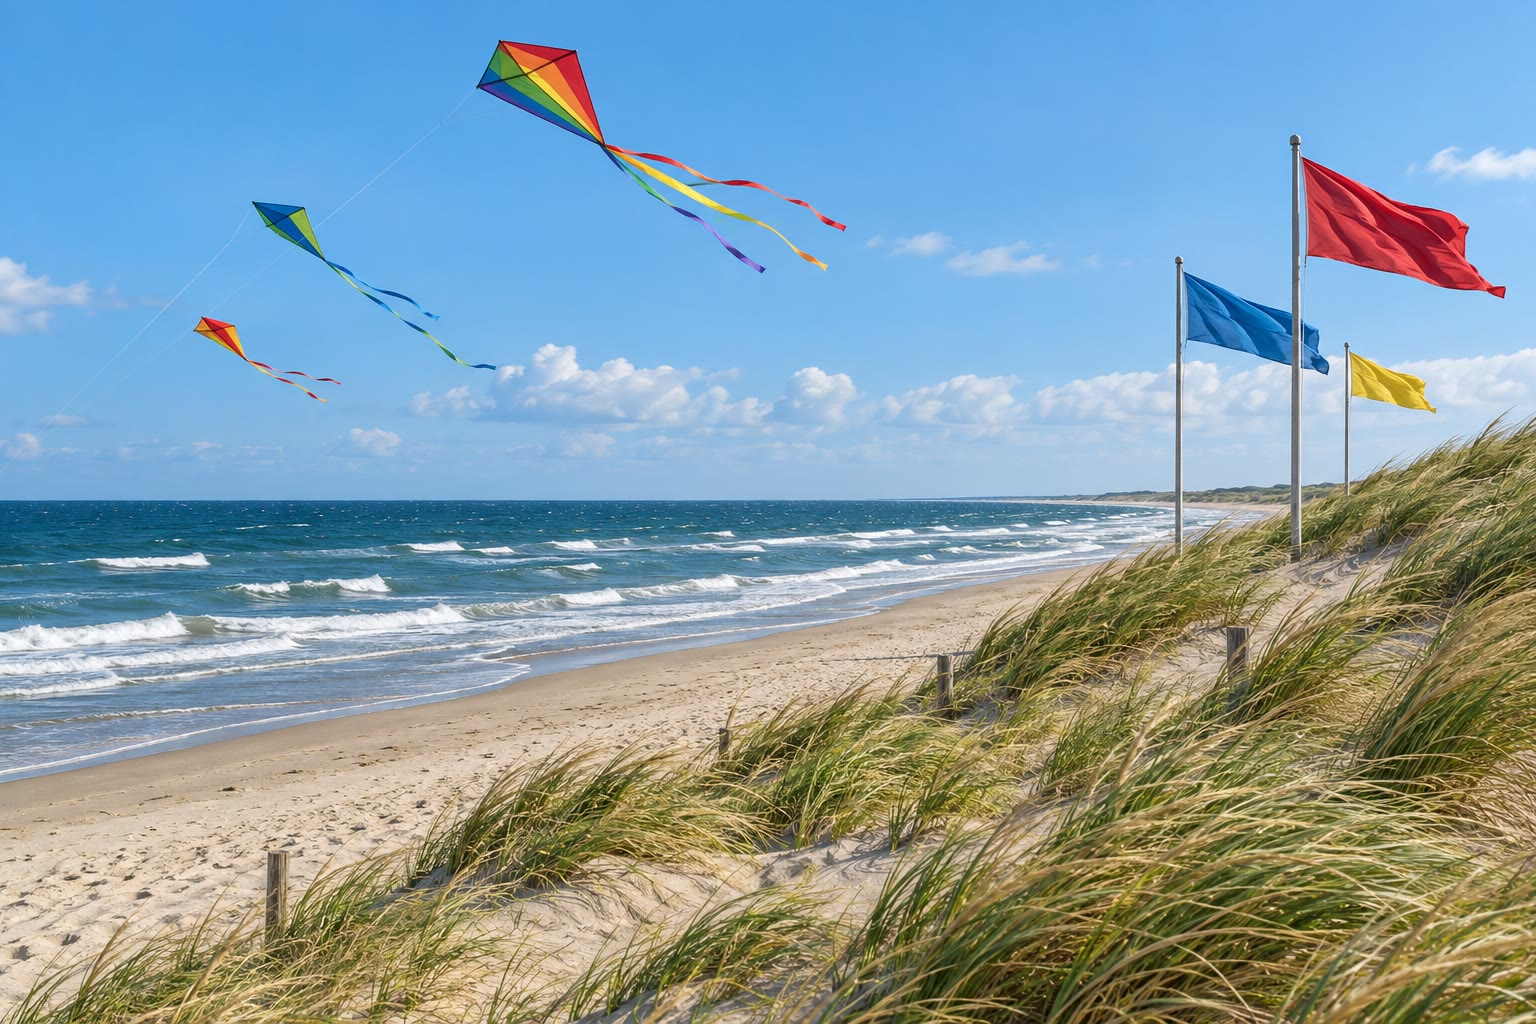
\includegraphics[width=0.55\linewidth]{images/book1/ai/g8-beach-kites.jpg}

{\small Cometas volando con el viento de la tarde en una playa
(ilustración generada por IA de una escena genérica).}
\label{fig:g8:winds-global-circulation:kites}
\end{omfigure}

\section{Los vientos globales}

Lo mismo ocurre a la escala de toda la Tierra. Cerca del \omterm{def:g3:continents-and-oceans:equator}{ecuador}, el aire,
muy calentado, sube; se extiende en altura hacia los \omterm{def:g3:continents-and-oceans:poles}{polos} y vuelve a bajar
hacia los \ang{30} de \omterm{def:g6:latitude-longitude:latitude}{latitud}. Como media a lo largo de muchos años, la
\omterm{def:g8:the-atmosphere:layers}{troposfera} de cada \omterm{def:g3:continents-and-oceans:equator}{hemisferio} gira en tres grandes \omterm{def:g8:winds-global-circulation:convection-cell}{células de convección}:
una del \omterm{def:g3:continents-and-oceans:equator}{ecuador} a unos \ang{30}, otra de unos \ang{30} a unos \ang{60}, y
otra de unos \ang{60} al \omterm{def:g3:continents-and-oceans:poles}{polo}. Los meteorólogos las llaman células de
Hadley, de Ferrel y polar. Sus límites se desplazan con las estaciones, y
la célula del medio es una media aproximada de muchas borrascas que pasan.
% ledger: mo:three-cells, mo:global-circ, nos:doldrums

Los vientos que soplan a ras de suelo irían directamente de las altas a las
bajas presiones si la Tierra no girara. Como la Tierra gira, el aire en
movimiento se desvía: hacia la derecha en el \omterm{def:g3:continents-and-oceans:equator}{hemisferio norte} y hacia la
izquierda en el \omterm{def:g3:continents-and-oceans:equator}{hemisferio sur}. Así que el aire que vuelve hacia el \omterm{def:g3:continents-and-oceans:equator}{ecuador}
no llega del norte, sino del nordeste en el \omterm{def:g3:continents-and-oceans:equator}{hemisferio norte} y del sudeste
en el \omterm{def:g3:continents-and-oceans:equator}{hemisferio sur}.
% ledger: mo:global-circ, nos:trade-winds

\begin{definition}[Los vientos globales]\label{def:g8:winds-global-circulation:global-winds}
Los vientos de superficie que soplan con más frecuencia en cada franja de
\omterm{def:g6:latitude-longitude:latitude}{latitud} son:
\begin{itemize}
  \item los \emph{alisios}\index{alisios}, entre el \omterm{def:g3:continents-and-oceans:equator}{ecuador} y unos
        \ang{30}, que soplan del nordeste en el \omterm{def:g3:continents-and-oceans:equator}{hemisferio norte} y del
        sudeste en el \omterm{def:g3:continents-and-oceans:equator}{hemisferio sur};
  \item los \emph{vientos del oeste}\index{vientos del oeste}, entre unos
        \ang{30} y \ang{60}, que soplan del oeste (del sudoeste en el
        \omterm{def:g3:continents-and-oceans:equator}{hemisferio norte}, del noroeste en el sur);
  \item los \emph{vientos polares del este}\index{vientos polares del este},
        entre unos \ang{60} y los \omterm{def:g3:continents-and-oceans:poles}{polos}, que soplan del este.
\end{itemize}
\end{definition}
% ledger: nos:trade-winds, mo:three-cells, mo:global-circ

\begin{omfigure}
\begin{tikzpicture}[font=\scriptsize, >={Stealth[length=1.8mm]}]
  \def\R{3}
  \fill[blue!8] (0,0) circle (\R);
  \draw (0,0) circle (\R);
  \draw[black!45] (-\R,0) -- (\R,0);
  \foreach \l in {-60,-30,30,60} {
    \pgfmathsetmacro{\y}{\R*sin(\l)}
    \pgfmathsetmacro{\x}{\R*cos(\l)}
    \draw[black!45, dashed] (-\x,\y) -- (\x,\y);}
  % surface winds: NE trades, SW westerlies, NE polar easterlies (north); mirrored south
  \foreach \x in {-1.8,-0.6,0.6,1.8} {
    \draw[->, omThm, line width=0.9pt] (\x+0.35,0.95) -- (\x-0.35,0.55);
    \draw[->, omThm, line width=0.9pt] (\x+0.35,-0.95) -- (\x-0.35,-0.55);}
  \foreach \x in {-1.2,0,1.2} {
    \draw[->, omDef, line width=0.9pt] (\x-0.35,1.7) -- (\x+0.35,2.02);
    \draw[->, omDef, line width=0.9pt] (\x-0.35,-1.7) -- (\x+0.35,-2.02);}
  \foreach \x in {-0.4,0.4} {
    \draw[->, omMeth, line width=0.9pt] (\x+0.25,2.85) -- (\x-0.25,2.65);
    \draw[->, omMeth, line width=0.9pt] (\x+0.25,-2.85) -- (\x-0.25,-2.65);}
  \node[fill=blue!8, inner sep=1pt] at (0,1.2) {alisios del nordeste};
  \node[fill=blue!8, inner sep=1pt] at (0,-1.2) {alisios del sudeste};
  \node[fill=blue!8, inner sep=1pt] at (0,2.3) {vientos del oeste};
  \node[fill=blue!8, inner sep=1pt] at (0,-2.3) {vientos del oeste};
  \node[anchor=south] at (0,\R+0.05) {vientos polares del este};
  \node[anchor=north] at (0,-\R-0.05) {vientos polares del este};
  % pressure belts on the left
  \foreach \l/\t in {90/{A: aire que baja}, 60/{B: aire que sube}, 30/{A: aire que baja, seco, desiertos}, 0/{B: aire que sube, nubes, lluvia}, -30/{A: aire que baja, seco, desiertos}, -60/{B: aire que sube}, -90/{A: aire que baja}} {
    \pgfmathsetmacro{\y}{\R*sin(\l)}
    \pgfmathsetmacro{\x}{\R*cos(\l)}
    \draw[black!40] (-\x-0.05,\y) -- (-3.35,\y);
    \node[anchor=east] at (-3.4,\y) {\t};}
  \foreach \l/\t in {60/{\ang{60} N}, 30/{\ang{30} N}, 0/{ecuador}, -30/{\ang{30} S}, -60/{\ang{60} S}} {
    \pgfmathsetmacro{\y}{\R*sin(\l)}
    \pgfmathsetmacro{\x}{\R*cos(\l)}
    \node[anchor=west, black!60] at (\x+0.05,\y) {\t};}
  % side view of the cells (height to the right), same latitude scale
  \begin{scope}[xshift=5.2cm]
    \draw[->] (0,-\R) -- (0,\R+0.3);
    \draw (0,-\R) -- (1.8,-\R);
    \node[anchor=north, align=center] at (0.9,-\R-0.05) {altura en la\\troposfera $\rightarrow$};
    \foreach \lo/\hi/\cw in {0/30/0, 30/60/1, 60/90/0, -30/0/1, -60/-30/0, -90/-60/1} {
      \pgfmathsetmacro{\ya}{\R*sin(\lo)}
      \pgfmathsetmacro{\yb}{\R*sin(\hi)}
      \pgfmathsetmacro{\yc}{(\ya+\yb)/2}
      \pgfmathsetmacro{\bb}{max(0.09,(\yb-\ya)/2-0.06)}
      \ifnum\cw=0
        \draw[black!70, line width=0.7pt, postaction={decorate}, decoration={markings,
          mark=at position 0.125 with {\arrow{Stealth[length=1.6mm]}}, mark=at position 0.375 with {\arrow{Stealth[length=1.6mm]}},
          mark=at position 0.625 with {\arrow{Stealth[length=1.6mm]}}, mark=at position 0.875 with {\arrow{Stealth[length=1.6mm]}}}]
          (0.9,\yc) ++(0.75,0) arc (0:360:0.75 and \bb);
      \else
        \draw[black!70, line width=0.7pt, postaction={decorate}, decoration={markings,
          mark=at position 0.125 with {\arrow{Stealth[length=1.6mm]}}, mark=at position 0.375 with {\arrow{Stealth[length=1.6mm]}},
          mark=at position 0.625 with {\arrow{Stealth[length=1.6mm]}}, mark=at position 0.875 with {\arrow{Stealth[length=1.6mm]}}}]
          (0.9,\yc) ++(0.75,0) arc (360:0:0.75 and \bb);
      \fi}
  \end{scope}
\end{tikzpicture}

{\small La \omterm{def:g8:winds-global-circulation:circulation}{circulación general}, simplificada. A la izquierda: las franjas
de altas (A) y bajas (B) presiones en el suelo. Sobre el \omterm{def:g3:continents-and-oceans:globe}{globo}: los vientos
de superficie, desviados por la rotación de la Tierra. A la derecha: las
tres \omterm{def:g8:winds-global-circulation:convection-cell}{células de convección} de cada \omterm{def:g3:continents-and-oceans:equator}{hemisferio} vistas de lado, a las mismas
\omterm{def:g6:latitude-longitude:latitude}{latitudes} (las células polares se dibujan muy finas porque la franja polar
es estrecha sobre el \omterm{def:g3:continents-and-oceans:globe}{globo}).}
% ledger: mo:three-cells, mo:global-circ, nos:trade-winds, nos:doldrums
\label{fig:g8:winds-global-circulation:cells}
\end{omfigure}

\begin{method}[Hallar el viento global a una latitud]\label{met:g8:winds-global-circulation:wind}
\begin{enumerate}
  \item Busca la franja: del \omterm{def:g3:continents-and-oceans:equator}{ecuador} a unos \ang{30}, de \ang{30} a
        \ang{60}, o de \ang{60} al \omterm{def:g3:continents-and-oceans:poles}{polo}.
  \item Busca hacia dónde se mueve el aire a ras de suelo en esa franja:
        hacia el \omterm{def:g3:continents-and-oceans:equator}{ecuador} en la primera y en la última franja, hacia el \omterm{def:g3:continents-and-oceans:poles}{polo}
        en la del medio.
  \item Desvía ese movimiento: hacia la derecha en el \omterm{def:g3:continents-and-oceans:equator}{hemisferio norte},
        hacia la izquierda en el \omterm{def:g3:continents-and-oceans:equator}{hemisferio sur}.
  \item Di de dónde viene el viento: los vientos se nombran según la
        dirección \emph{desde la que} soplan.
\end{enumerate}
\end{method}

\begin{example}[El viento a \ang{40} sur]\label{ex:g8:winds-global-circulation:40s}
A \ang{40} S estamos en la franja del medio, entre \ang{30} y \ang{60}.
Allí el aire se mueve a ras de suelo hacia el \omterm{def:g3:continents-and-oceans:poles}{polo}, es decir, hacia el
sur. En el \omterm{def:g3:continents-and-oceans:equator}{hemisferio sur} se desvía hacia la izquierda: para un aire que
va hacia el sur, la izquierda es el este, así que el aire acaba moviéndose
hacia el sudeste. Por tanto, viene del noroeste: es uno de los \omterm{def:g8:winds-global-circulation:global-winds}{vientos del
oeste}, que sopla del noroeste.
\end{example}
% ledger: mo:three-cells, mo:global-circ

Cerca del \omterm{def:g3:continents-and-oceans:equator}{ecuador}, donde se encuentran los \omterm{def:g8:winds-global-circulation:global-winds}{alisios} de los dos \omterm{def:g3:continents-and-oceans:equator}{hemisferios},
los vientos amainan: los marinos llamaron a esta franja de calma las
\emph{calmas ecuatoriales}. Allí el aire cálido y húmedo sube, se enfría y
da chubascos y \omterm{def:g5:natural-hazards:storm}{tormentas} persistentes. Hacia los \ang{30}, bajo el aire
que baja, los vientos son flojos y la \omterm{def:g4:clouds-rain-snow:precipitation}{lluvia} es escasa.
% ledger: nos:doldrums

\begin{definition}[Circulación general de la atmósfera]\label{def:g8:winds-global-circulation:circulation}
La \emph{circulación general}\index{circulacion general@circulación general}
de la atmósfera es el movimiento de aire a gran escala alrededor del
planeta, que se ve cuando se promedian los vientos a lo largo de muchos
años. Lleva calor del \omterm{def:g3:continents-and-oceans:equator}{ecuador} hacia los \omterm{def:g3:continents-and-oceans:poles}{polos}, y vapor de agua de una
franja de \omterm{def:g6:latitude-longitude:latitude}{latitud} a otra.
\end{definition}
% ledger: mo:global-circ

\section{La circulación general y las zonas climáticas}

La \omterm{def:g8:winds-global-circulation:circulation}{circulación general} explica buena parte del \omterm{def:g2:drawing-to-map:map}{mapa} de los \omterm{def:g5:weather-and-climate:climate}{climas}. Donde el
aire sube, cerca del \omterm{def:g3:continents-and-oceans:equator}{ecuador}, se enfría y su vapor de agua se convierte en
\omterm{def:g4:clouds-rain-snow:cloud}{nubes}: la \omterm{def:g4:clouds-rain-snow:precipitation}{lluvia} es frecuente, y crecen las \omterm{def:g5:weather-and-climate:rainforest}{selvas tropicales}. Donde el
aire baja, hacia los \ang{30} norte y sur, se calienta al descender, sus
\omterm{def:g4:clouds-rain-snow:cloud}{nubes} se disipan y la \omterm{def:g4:clouds-rain-snow:precipitation}{lluvia} es escasa: los grandes \omterm{def:g5:weather-and-climate:desert}{desiertos} cálidos, como
el Sáhara, están en estas franjas. En las \omterm{def:g6:latitude-longitude:latitude}{latitudes} medias, los \omterm{def:g8:winds-global-circulation:global-winds}{vientos del
oeste} traen una borrasca tras otra, con \omterm{def:g4:clouds-rain-snow:precipitation}{lluvia} en todas las estaciones.
% ledger: nos:doldrums, mo:three-cells, mo:global-circ

\begin{omfigure}
\begin{minipage}[c]{0.42\linewidth}\centering
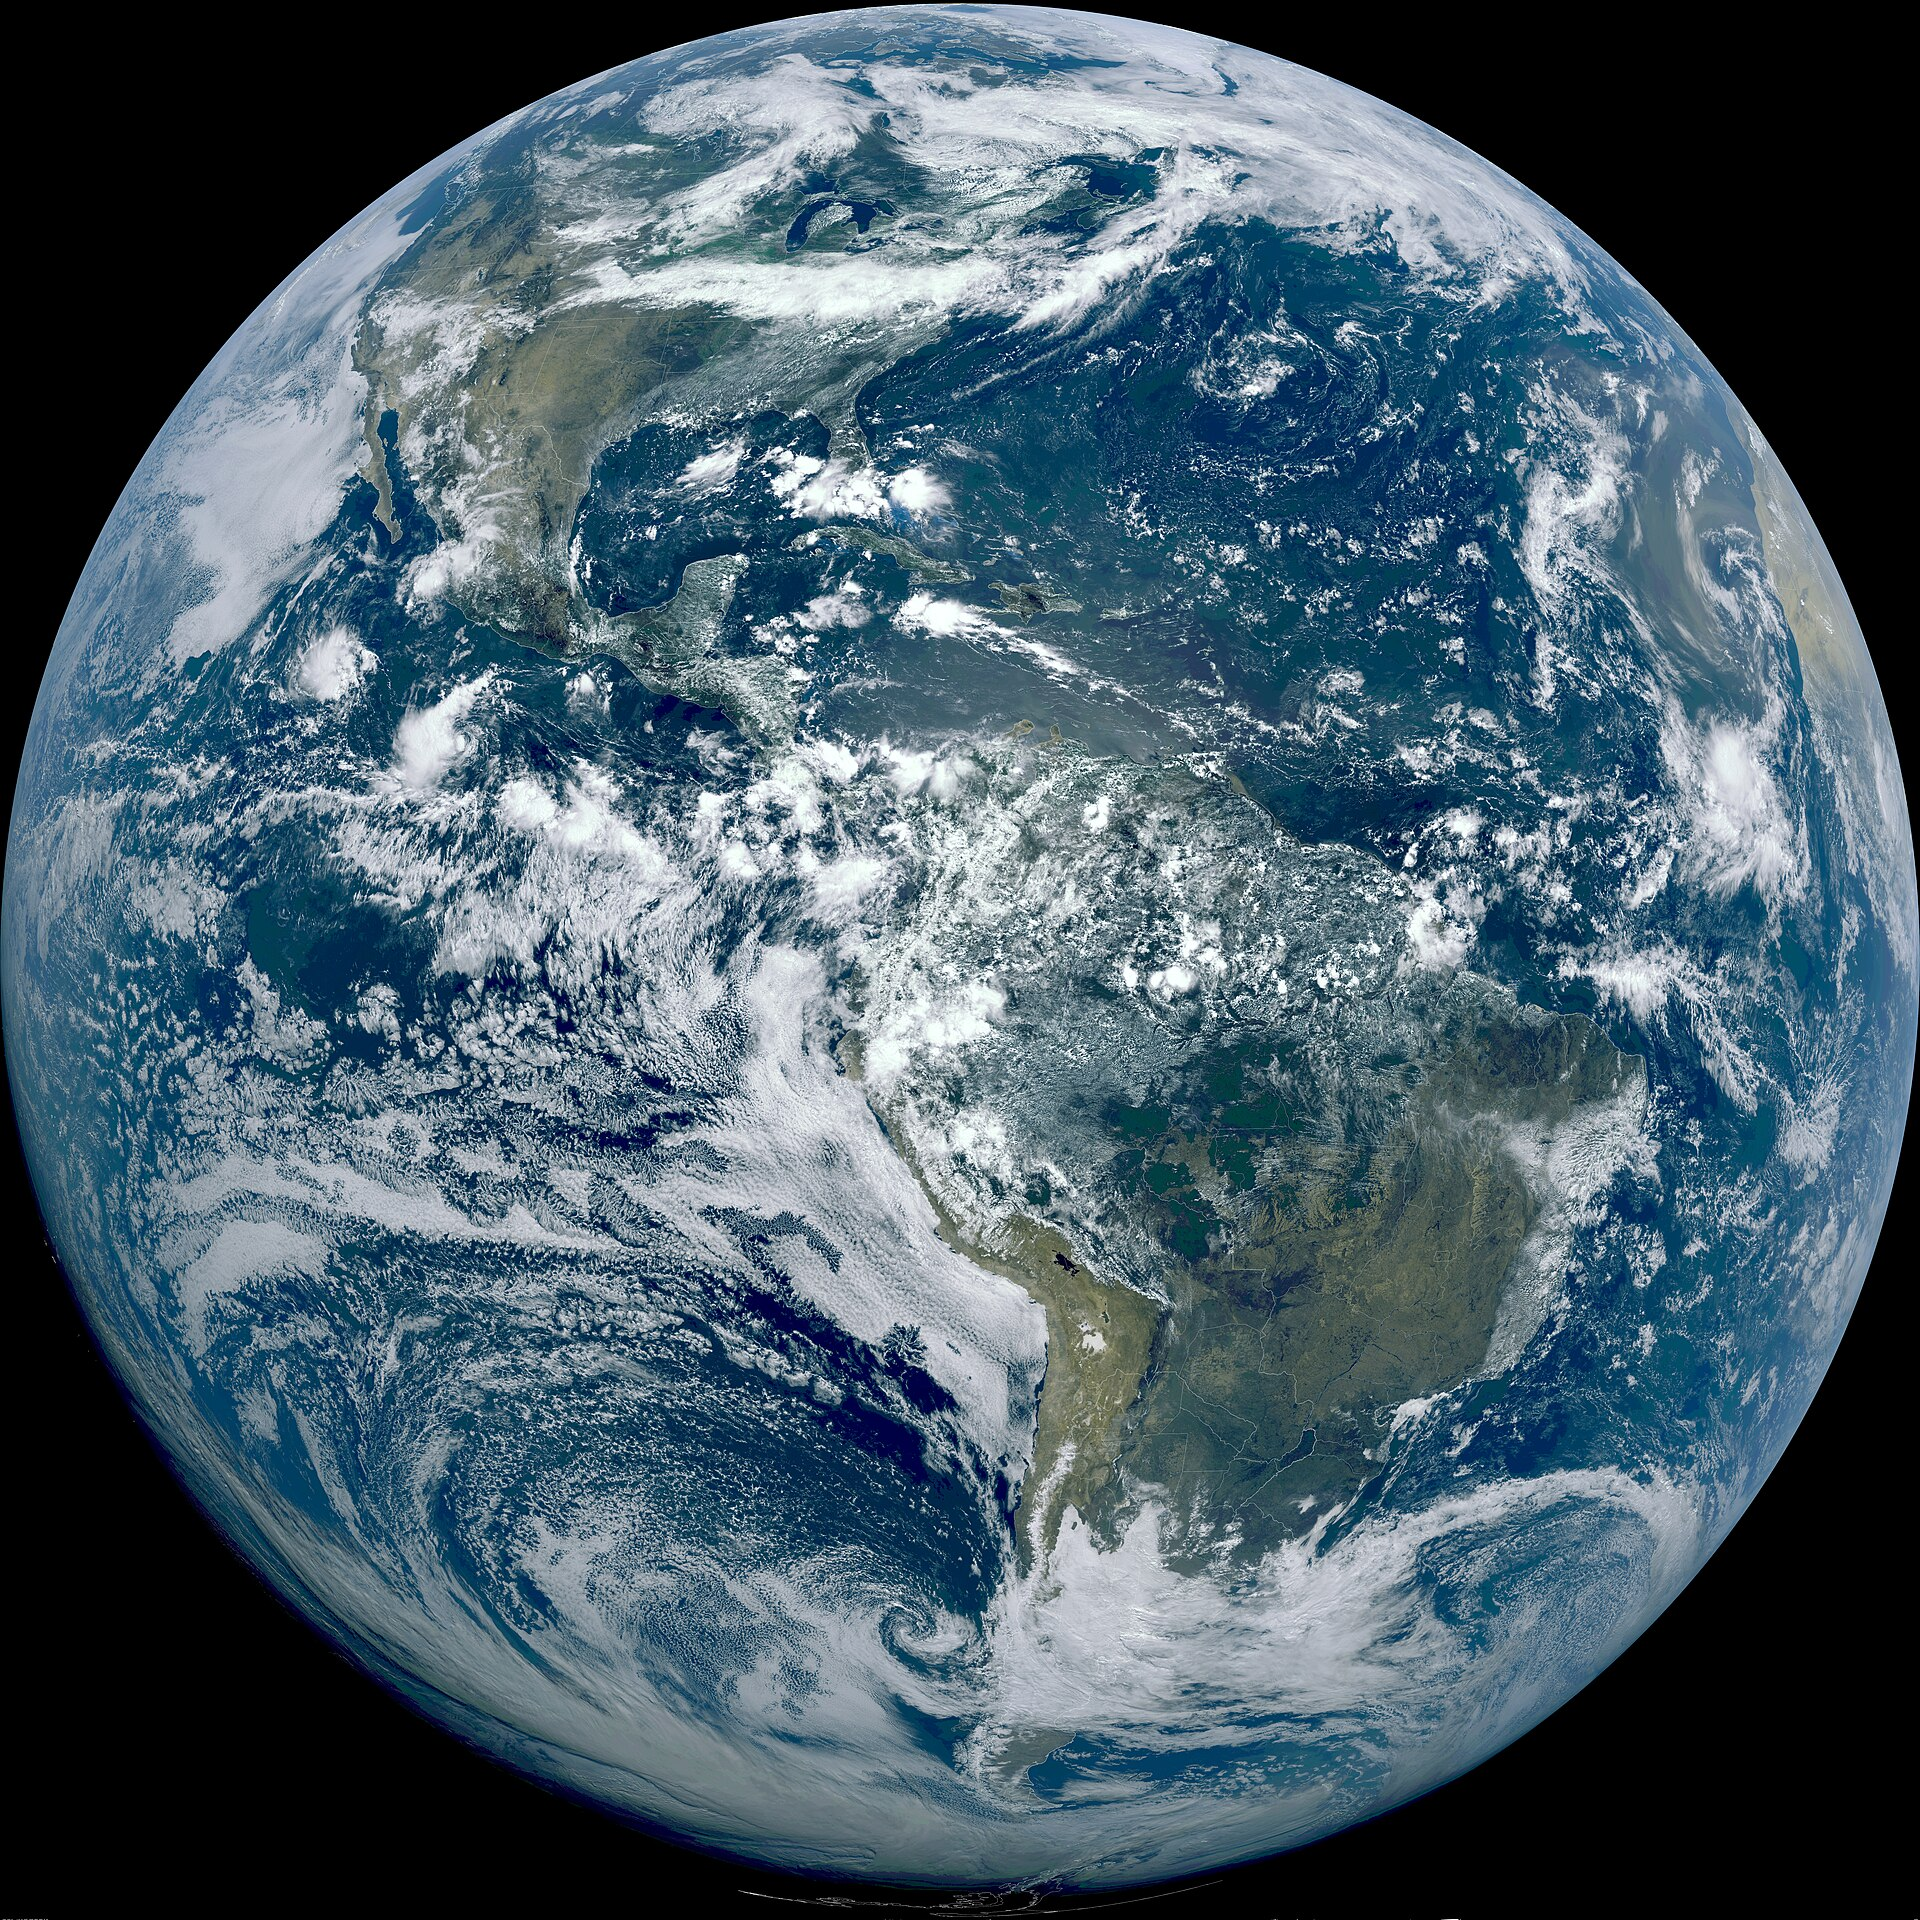
\includegraphics[width=\linewidth]{images/book1/g8-goes-full-disk.jpg}
\end{minipage}\hfill
\begin{minipage}[c]{0.54\linewidth}\raggedright
{\small América vista por el satélite meteorológico GOES-16, muy por encima
del \omterm{def:g3:continents-and-oceans:equator}{ecuador}, el 26~de julio de 2022. Se han formado muchas \omterm{def:g4:clouds-rain-snow:cloud}{nubes} sobre los
\omterm{def:g5:weather-and-climate:tropics}{trópicos} y la selva amazónica, donde sube el aire cálido y húmedo; muy al
sur, en el invierno austral, las borrascas de los \omterm{def:g8:winds-global-circulation:global-winds}{vientos del oeste} se
arremolinan sobre el \omterm{def:g2:water-on-earth:ocean}{océano}. NOAA (dominio público, vía Wikimedia Commons).}
\end{minipage}
% ledger: commons:goes16, nos:doldrums
\label{fig:g8:winds-global-circulation:goes}
\end{omfigure}

\begin{example}[Cuatro ciudades, cuatro franjas]\label{ex:g8:winds-global-circulation:four-towns}
Las cuatro ciudades de los \omterm{def:g5:weather-and-climate:climate-chart}{climogramas} del \cref{ch:g5:weather-and-climate}
están todas en el \omterm{def:g3:continents-and-oceans:equator}{hemisferio norte}, a \omterm{def:g6:latitude-longitude:latitude}{latitudes} muy distintas. Su \omterm{def:g4:clouds-rain-snow:precipitation}{lluvia} y
su \omterm{def:g4:clouds-rain-snow:precipitation}{nieve} anuales siguen las franjas de la \omterm{def:g8:winds-global-circulation:circulation}{circulación general} (gráfico de
abajo). Hilo, a \ang{20}\,N, está en una isla de la franja de los \omterm{def:g8:winds-global-circulation:global-winds}{alisios},
en medio del \omterm{def:g2:water-on-earth:ocean}{océano}, donde los \omterm{def:g8:winds-global-circulation:global-winds}{alisios} se cargan de vapor de agua: allí
caen unos \qty{3000}{mm} al año. Phoenix, a \ang{33}\,N, está cerca de los
\ang{30}, bajo el aire que baja: menos de \qty{200}{mm}. Seattle, a
\ang{47}\,N, está en los \omterm{def:g8:winds-global-circulation:global-winds}{vientos del oeste}, cuyas borrascas traen unos
\qty{1000}{mm} al año, la mayor parte de otoño a primavera. Utqiaġvik, a
\ang{71}\,N, está bajo el aire frío que baja cerca del \omterm{def:g3:continents-and-oceans:poles}{polo}: menos de
\qty{150}{mm}, un \omterm{def:g5:weather-and-climate:desert}{desierto} frío.
% ledger: data:b1-noaa-normals (totals from figdata/grade-5/climate_charts.py, re-read in figdata/grade-8/rain_by_belt.py), mo:three-cells, nos:doldrums
\end{example}

\begin{omfigure}
\begin{tikzpicture}
\begin{axis}[xbar, width=0.82\linewidth, height=6.4cm, bar width=9pt,
  xmin=0, xmax=3600, ymin=0, ymax=90, ytick={0,30,60,90},
  yticklabels={$0^\circ$, $30^\circ$\,N, $60^\circ$\,N, $90^\circ$\,N},
  xlabel={lluvia y nieve en un año (mm)}, ylabel={latitud},
  axis x line=bottom, axis y line=left, axis line style={-},
  tick label style={font=\scriptsize}, label style={font=\small},
  xtick={0,1000,2000,3000}, scaled x ticks=false, clip=false,
  point meta=explicit symbolic, nodes near coords,
  nodes near coords style={font=\scriptsize, anchor=west}]
  \draw[black!35, dashed] (axis cs:0,30) -- (axis cs:3600,30);
  \draw[black!35, dashed] (axis cs:0,60) -- (axis cs:3600,60);
  \node[font=\scriptsize, black!60, anchor=south east] at (axis cs:3600,1) {aire que sube: lluvia};
  \node[font=\scriptsize, black!60, anchor=south east] at (axis cs:3600,30) {aire que baja: seco};
  \node[font=\scriptsize, black!60, anchor=south east] at (axis cs:3600,60) {aire que sube: lluvia};
  \node[font=\scriptsize, black!60, anchor=north east] at (axis cs:3600,90) {aire que baja: seco};
  \addplot[fill=blue!35, draw=blue!60!black] table[x=total_mm, y=lat, meta=name] {figdata/out/grade-8-rain_by_belt-stations.dat};
\end{axis}
\end{tikzpicture}

{\small \omterm{def:g4:clouds-rain-snow:precipitation}{Lluvia} y \omterm{def:g4:clouds-rain-snow:precipitation}{nieve} anuales (medias de 1991--2020) de las cuatro
ciudades de los \omterm{def:g5:weather-and-climate:climate-chart}{climogramas}, colocadas a su \omterm{def:g6:latitude-longitude:latitude}{latitud}. Las ciudades húmedas
están donde el aire sube, cerca del \omterm{def:g3:continents-and-oceans:equator}{ecuador} y hacia los \ang{60}; las
secas, donde baja, hacia los \ang{30} y cerca del \omterm{def:g3:continents-and-oceans:poles}{polo}. Normales
climáticas de la NOAA.}
% ledger: data:b1-noaa-normals, mo:three-cells (figdata/grade-8/rain_by_belt.py)
\end{omfigure}

Cuatro ciudades no son más que cuatro puntos: las \omterm{def:g1:landscapes-around-us:landform}{montañas}, las \omterm{def:g1:landscapes-around-us:water}{costas} y
los \omterm{def:g2:water-on-earth:ocean}{mares} fríos o cálidos también cambian la cantidad de \omterm{def:g4:clouds-rain-snow:precipitation}{lluvia} que recibe
un lugar. Las franjas dan el esquema general del \omterm{def:g2:drawing-to-map:map}{mapa} de los \omterm{def:g5:weather-and-climate:climate}{climas}, no la
\omterm{def:g4:clouds-rain-snow:precipitation}{lluvia} de cada ciudad.

\section{Ejercicios}

\begin{exercise}[$\star$]\label{exo:g8:winds-global-circulation:1}
Di qué viento global sopla con más frecuencia: (a) a \ang{15} norte;
(b) a \ang{45} sur; (c) a \ang{75} norte; (d) a \ang{20} sur. Da cada vez
su dirección.
\end{exercise}

\begin{exercise}[$\star$]\label{exo:g8:winds-global-circulation:2}
Completa cada frase. (a) El aire cálido \dots\ y el aire frío \dots.
(b) Bajo el aire que sube, la presión en el suelo es \dots. (c) En el
suelo, el viento sopla de las presiones \dots\ hacia las presiones \dots.
(d) En el \omterm{def:g3:continents-and-oceans:equator}{hemisferio norte}, la rotación de la Tierra desvía el aire en
movimiento hacia la \dots.
\end{exercise}

\begin{exercise}[$\star$]\label{exo:g8:winds-global-circulation:3}
¿Verdadero o falso? Corrige las frases falsas. (a) Una \omterm{def:g8:winds-global-circulation:breezes}{brisa marina} sopla
de la tierra hacia el \omterm{def:g2:water-on-earth:ocean}{mar}. (b) De día, la tierra se calienta más deprisa
que el \omterm{def:g2:water-on-earth:ocean}{mar}. (c) Los \omterm{def:g8:winds-global-circulation:global-winds}{alisios} soplan del oeste. (d) Muchos grandes \omterm{def:g5:weather-and-climate:desert}{desiertos}
están cerca de los \ang{30} de \omterm{def:g6:latitude-longitude:latitude}{latitud}.
\end{exercise}

\begin{exercise}[$\star$]\label{exo:g8:winds-global-circulation:4}
Dibuja una \omterm{def:g1:landscapes-around-us:water}{costa} con el \omterm{def:g2:water-on-earth:ocean}{mar} a la izquierda y la tierra a la derecha. Añade
el Sol y dibuja luego con flechas el circuito de aire de la \omterm{def:g8:winds-global-circulation:breezes}{brisa marina}.
Marca con A y B dónde es alta y dónde es baja la presión en el suelo.
\end{exercise}

\begin{exercise}[$\star\star$]\label{exo:g8:winds-global-circulation:5}
Usa la tabla de los haces de este capítulo. (a) A \ang{45}, ¿cuánto más
suelo cubre un haz que en el \omterm{def:g3:continents-and-oceans:equator}{ecuador}? (b) ¿Qué porcentaje de la energía
del \omterm{def:g3:continents-and-oceans:equator}{ecuador} recibe cada metro cuadrado a \ang{60}? (c) ¿Y a \ang{75}?
(d) Explica en una frase por qué los \omterm{def:g3:continents-and-oceans:poles}{polos} son fríos.
\end{exercise}

\begin{exercise}[$\star\star$]\label{exo:g8:winds-global-circulation:6}
Un barco navega rumbo al sur a través del \omterm{def:g3:continents-and-oceans:equator}{hemisferio norte} y después del
\omterm{def:g3:continents-and-oceans:equator}{hemisferio sur}. (a) ¿Qué vientos encuentra, en orden, de \ang{70} N a
\ang{70} S? (b) ¿Dónde es probable que encuentre calma y chubascos
frecuentes? (c) ¿Dónde son los vientos flojos y la \omterm{def:g4:clouds-rain-snow:precipitation}{lluvia} escasa?
\end{exercise}

\begin{exercise}[$\star\star$]\label{exo:g8:winds-global-circulation:7}
En una playa hace \qty{31}{\degreeCelsius} sobre la \omterm{def:g3:stones-pebbles-sand:sand}{arena} a las 3 de la
tarde y \qty{22}{\degreeCelsius} sobre el \omterm{def:g2:water-on-earth:ocean}{mar}. A las 3 de la madrugada hace
\qty{17}{\degreeCelsius} en tierra y \qty{21}{\degreeCelsius} sobre el \omterm{def:g2:water-on-earth:ocean}{mar}.
(a) ¿Qué está más caliente a las 3 de la tarde? ¿Hacia dónde sopla el
viento? (b) ¿Y a las 3 de la madrugada? (c) ¿Cuántos grados cambia la
temperatura de la tierra entre las dos horas? ¿Y la del \omterm{def:g2:water-on-earth:ocean}{mar}? (d) Explica
la diferencia.
\end{exercise}

\begin{exercise}[$\star\star$]\label{exo:g8:winds-global-circulation:8}
El aire se mueve desde la franja de altas presiones de los \ang{30} N
hacia el \omterm{def:g3:continents-and-oceans:equator}{ecuador}. (a) Sin la rotación de la Tierra, ¿de qué dirección
soplaría? (b) ¿Hacia qué lado lo desvía la rotación en este \omterm{def:g3:continents-and-oceans:equator}{hemisferio}?
(c) ¿De qué dirección sopla entonces? (d) Responde a las mismas tres
preguntas para el aire que se mueve hacia el \omterm{def:g3:continents-and-oceans:equator}{ecuador} desde los \ang{30} S.
\end{exercise}

\begin{exercise}[$\star\star$]\label{exo:g8:winds-global-circulation:9}
Explica, paso a paso, por qué llueve tan a menudo cerca del \omterm{def:g3:continents-and-oceans:equator}{ecuador}: usa
las palabras \emph{calentado}, \emph{sube}, \emph{se enfría}, \emph{\omterm{def:g4:clouds-rain-snow:cloud}{nubes}}.
Después explica por qué hay un \omterm{def:g5:weather-and-climate:desert}{desierto} hacia los \ang{25} N en el norte de
África: usa las palabras \emph{baja}, \emph{altas presiones}, \emph{seco}.
\end{exercise}

\begin{exercise}[$\star\star$]\label{exo:g8:winds-global-circulation:10}
Un velero sale de un puerto situado a \ang{40} N, en la \omterm{def:g1:landscapes-around-us:water}{costa} occidental de
Europa, hacia el Caribe, a \ang{15} N. (a) ¿Qué viento encontraría a
\ang{40} N? ¿Le ayudaría a navegar hacia el oeste? (b) ¿Por qué debería el
barco navegar primero hacia el sur? (c) ¿Qué viento lo lleva hacia el
oeste, y entre qué \omterm{def:g6:latitude-longitude:latitude}{latitudes}? (d) Para el viaje de vuelta a Europa, ¿qué
viento debería buscar el barco, y a qué \omterm{def:g6:latitude-longitude:latitude}{latitud}?
\end{exercise}

\begin{exercise}[$\star\star\star$]\label{exo:g8:winds-global-circulation:11}
A la \omterm{def:g6:latitude-longitude:latitude}{latitud} $L$, un haz de luz solar a mediodía en un equinoccio cubre
$1 \div
\cos L$ veces el suelo que cubre en el \omterm{def:g3:continents-and-oceans:equator}{ecuador} (con una calculadora,
$\cos 60^\circ = 0.5$). (a) Comprueba el valor para \ang{60}. (b) Usando
$\cos 30^\circ \approx 0.866$, comprueba el valor para \ang{30},
redondeado a dos decimales. (c) Supón que un panel solar colocado en
horizontal recibe \qty{1000}{W} por cada metro cuadrado a mediodía en el
\omterm{def:g3:continents-and-oceans:equator}{ecuador} ese día. ¿Cuánto recibiría, más o menos, el mismo panel a
\ang{30}? ¿Y a \ang{60}?
\end{exercise}

\begin{exercise}[$\star\star\star$]\label{exo:g8:winds-global-circulation:12}
En cada \omterm{def:g3:continents-and-oceans:equator}{hemisferio}, la \omterm{def:g8:winds-global-circulation:circulation}{circulación general} tiene tres células. (a) Dibuja
una vista lateral del \omterm{def:g3:continents-and-oceans:equator}{hemisferio norte}, con el \omterm{def:g3:continents-and-oceans:equator}{ecuador} abajo y el \omterm{def:g3:continents-and-oceans:poles}{polo}
arriba, y las tres células como circuitos; indica dónde sube y dónde baja
el aire. (b) Marca las franjas de altas y bajas presiones en el suelo.
(c) Añade los vientos de superficie de cada célula, desviados hacia la
derecha. (d) Usa tu dibujo para explicar por qué los \omterm{def:g8:winds-global-circulation:global-winds}{vientos del oeste}
soplan hacia el nordeste.
\end{exercise}

\section{Problema: navegar con los alisios}

\begin{problem}[{Problema de fin de semana --- un velero cruza el Atlántico
de Cabo Verde a Barbados con el alisio del nordeste; se mide la ruta en el
mapa, se lee el viento y se calcula la duración de la travesía}]
\label{pb:g8:winds-global-circulation:1}
% ledger: data:b1-ne-places, earth:Rmean, nos:trade-winds (figdata/grade-8/trade_route.py; the speed is exercise data)
Un velero sale de Praia, en las islas de Cabo Verde, hacia Bridgetown, en
Barbados. El \omterm{def:g2:drawing-to-map:map}{mapa} muestra la ruta y el alisio.

\begin{center}
\begin{tikzpicture}
\begin{axis}[ommap, width=12cm, xmin=-75, xmax=-5, ymin=0, ymax=35, axis equal image,
  xtick={-70,-60,-50,-40,-30,-20,-10}, ytick={0,10,20,30},
  tick label style={font=\scriptsize},
  xlabel={longitud (negativa = oeste)}, ylabel={latitud (norte)},
  label style={font=\small}, clip mode=individual]
  \addplot[fill=omLithAlluv, draw=black!60, line width=0.3pt] table {figdata/out/grade-8-trade_route-land.dat};
  \addplot[quiver={u=\thisrow{dlon}, v=\thisrow{dlat}}, -{Stealth[length=1.6mm]}, omThm!80, line width=0.7pt]
    table[x=lon, y=lat] {figdata/out/grade-8-trade_route-trades.dat};
  \addplot[omDef, line width=1.3pt, dashed] table {figdata/out/grade-8-trade_route-route.dat};
  \addplot[only marks, mark=*, mark size=2pt, black] table[x=lon, y=lat] {figdata/out/grade-8-trade_route-ports.dat};
  \node[anchor=north, font=\scriptsize\bfseries, fill=white, inner sep=1pt] at (axis cs:-59.6,12.2) {Bridgetown};
  \node[anchor=south, font=\scriptsize\bfseries, fill=white, inner sep=1pt] at (axis cs:-23.5,15.8) {Praia};
\end{axis}
\end{tikzpicture}
\end{center}

\noindent\textbf{Parte I --- La ruta.}\par\nopagebreak
\begin{enumerate}[beginpenalty=10000]
  \item Praia está a \ang{14.9} N, \ang{23.5} O; Bridgetown, a
        \ang{13.1} N, \ang{59.6} O. ¿Cuántos grados de \omterm{def:g6:latitude-longitude:longitude}{longitud} los
        separan?
  \item Los dos puertos están cerca de los \ang{14} N. A lo largo de este
        \omterm{def:g6:latitude-longitude:latitude}{paralelo}, un grado de \omterm{def:g6:latitude-longitude:longitude}{longitud} mide unos \qty{108}{km}. ¿Cuántos
        kilómetros mide, más o menos, la travesía? Redondea a la centena
        más cercana.
  \item Medida con exactitud sobre la Tierra redonda, la ruta más corta
        mide \qty{3896}{km}. ¿Es la respuesta de la pregunta 2 una buena
        estimación?
  \item ¿Están los puertos en la franja de los \omterm{def:g8:winds-global-circulation:global-winds}{alisios}? Explícalo.
\end{enumerate}

\noindent\textbf{Parte II --- El viento.}\par\nopagebreak
\begin{enumerate}[resume, beginpenalty=10000]
  \item ¿De qué dirección sopla aquí el alisio?
  \item El barco navega hacia el oeste. ¿El viento lo empuja hacia
        delante, hacia atrás o de lado? Explícalo con el \omterm{def:g2:drawing-to-map:map}{mapa}.
  \item ¿Por qué el alisio sopla en la misma dirección casi todos los días
        de la travesía?
  \item En el viaje de vuelta a Europa, ¿por qué no debería el capitán
        intentar navegar hacia el este a lo largo de los \ang{14} N?
\end{enumerate}

\noindent\textbf{Parte III --- La travesía.}\par\nopagebreak
\begin{enumerate}[resume, beginpenalty=10000]
  \item Supón que el barco avanza de media \qty{7}{km} por hora. ¿Cuántos
        kilómetros recorre en un día de 24 horas?
  \item Si el viento amainara durante 3 días por el camino, ¿cuántos
        kilómetros de avance perdería el barco?
  \item Con un alisio constante, ¿cuántos días necesita el barco para
        recorrer \qty{3896}{km}? Redondea a un decimal.
  \item Redondeando al día entero, ¿cuánto dura la travesía? ¿Es más o
        menos de un mes?
\end{enumerate}
\end{problem}
